\documentclass[../../main.tex]{subfiles}
\begin{document}

{\bf [解答]}

\begin{figure}[htb]
  \centering
  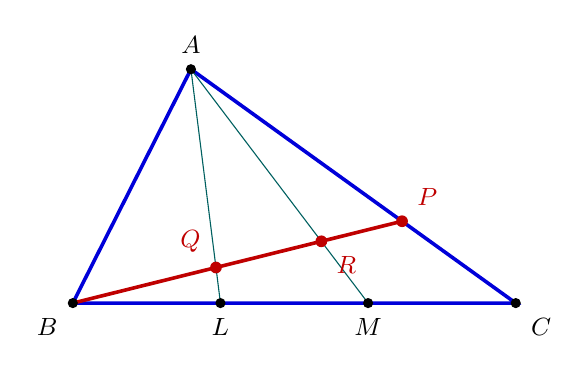
\begin{tikzpicture}[x=1.25cm, y=1.1cm, every node/.style={font=\small}]
    % P is on AC with AP/AC=0.65; L and M trisect BC.
    \coordinate (A) at (1.2,2.7);
    \coordinate (B) at (0,0);
    \coordinate (C) at (4.5,0);
    \coordinate (L) at (1.5,0);
    \coordinate (M) at (3,0);
    \coordinate (P) at (3.345,0.945);
    \coordinate (Q) at (intersection of B--P and A--L);
    \coordinate (R) at (intersection of B--P and A--M);
    \draw[line width=1.3pt, blue!85!black] (A)--(B)--(C)--cycle;
    \draw[thin, teal!75!black] (A)--(L) (A)--(M);
    \draw[line width=1.3pt, red!75!black] (B)--(P);
    \node[circle, fill, inner sep=1.3pt] at (A) {}; \node[above=2pt] at (A) {$A$};
    \node[circle, fill, inner sep=1.3pt] at (B) {}; \node[below left=2pt] at (B) {$B$};
    \node[circle, fill, inner sep=1.3pt] at (C) {}; \node[below right=2pt] at (C) {$C$};
    \node[circle, fill, inner sep=1.3pt] at (L) {}; \node[below=2pt] at (L) {$L$};
    \node[circle, fill, inner sep=1.3pt] at (M) {}; \node[below=2pt] at (M) {$M$};
    \node[circle, fill=red!75!black, inner sep=1.5pt] at (P) {}; \node[red!75!black, above right=2pt] at (P) {$P$};
    \node[circle, fill=red!75!black, inner sep=1.5pt] at (Q) {}; \node[red!75!black, above left=2pt] at (Q) {$Q$};
    \node[circle, fill=red!75!black, inner sep=1.5pt] at (R) {}; \node[red!75!black, below right=2pt] at (R) {$R$};
  \end{tikzpicture}
  \caption{$BC$ の三等分点 $L,M$ と $BP$ 上の点 $Q,R$}
  \label{fig:1964_3_triangle}
\end{figure}

\subparagraph{(イ)}

点$B$を始点とするベクトルを取り，点$X$に対して$\overrightarrow{BX}=\vec{x}$と定めると，
$\vec{a}, \vec{c}$は一次独立である．

$\vec{q}, \vec{r}$ はそれぞれ$AL,BP$と$AM,BP$上だから，ふた通りで
\begin{align}
  &
  \begin{cases}
    \vec{q} = k \vec{p} = (1-t)\vec{a} + t\vec{l} \\
    \vec{r} = K' \vec{p} = (1-t')\vec{a} + t'\vec{m}
  \end{cases} \\
  \therefore
  &
  \begin{cases}
    \vec{q} = k [(1-p)\vec{a} + p\vec{c}] = (1-t)\vec{a} + t \dfrac{1}{3}\vec{c} \\
    \vec{r} = K [(1-p)\vec{a} + p\vec{c}] = (1-t')\vec{a} + t' \dfrac{2}{3}\vec{c}
  \end{cases}
\end{align}
と書ける．これをといて $k = \dfrac{1}{2p+1}$, $k' = \dfrac{2}{p+2}$ だから
\begin{align}
  |BQ| : |QR| : |RP|
  &= k : k'-k : 1-k' \\
  &= \dfrac{1}{2p+1} : \dfrac{2}{p+2} - \dfrac{1}{2p+1} : 1 - \dfrac{2}{p+2} \\
  &= p+2 : 3p : p(2p+1)
\end{align}
である．

\begin{figure}[htb]
  \centering
  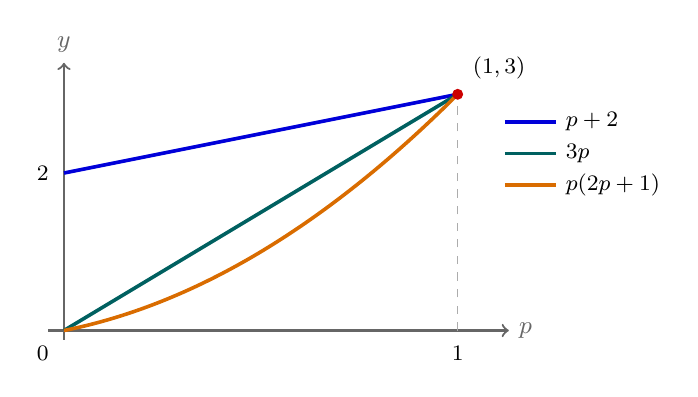
\begin{tikzpicture}[x=5cm, y=1cm, every node/.style={font=\small}]
    \draw[->, thick, gray!80!black] (-0.04,0)--(1.13,0) node[right] {$p$};
    \draw[->, thick, gray!80!black] (0,-0.12)--(0,3.4) node[above] {$y$};
    \draw[dashed, gray!65] (1,0)--(1,3.1);
    \draw[line width=1.3pt, blue!85!black] (0,2)--(1,3);
    \draw[line width=1.3pt, teal!75!black] (0,0)--(1,3);
    \draw[line width=1.3pt, orange!85!black, domain=0:1,
    samples=60, smooth] plot (\x,{\x*(2*\x+1)});
    \node[circle, fill=red!80!black, inner sep=1.4pt] at (1,3) {};
    \node[below left=2pt, font=\footnotesize] at (0,0) {$0$};
    \node[below=2pt, font=\footnotesize] at (1,0) {$1$};
    \node[left=2pt, font=\footnotesize] at (0,2) {$2$};
    \node[above right=2pt, font=\footnotesize] at (1,3) {$(1,3)$};
    \draw[line width=1.3pt, blue!85!black] (1.12,2.65)--(1.25,2.65);
    \node[right, font=\footnotesize] at (1.25,2.65) {$p+2$};
    \draw[line width=1.3pt, teal!75!black] (1.12,2.25)--(1.25,2.25);
    \node[right, font=\footnotesize] at (1.25,2.25) {$3p$};
    \draw[line width=1.3pt, orange!85!black] (1.12,1.85)--(1.25,1.85);
    \node[right, font=\footnotesize] at (1.25,1.85) {$p(2p+1)$};
  \end{tikzpicture}
  \caption{$0\le p\le1$ における三つの線分長の比の大小}
  \label{fig:1964_3_ratios}
\end{figure}

$0\le p\le 1$の時，$y=p+2,y=3p,y=p(2p+1)$のグラフは上図であり，
\begin{align}
  p(2p+1) \leqq 3p \leqq p+2
  \therefore
  |RP| \leqq |QR| \leqq |BQ|
\end{align}
となる．等号成立は $p=0$ (左だけ)又は $p=1$ の時で，それぞれ$P=A,P=C$となる．

\subparagraph{(ロ)}

3辺の長さを $a = p+2$, $b = 3p$, $c = 2p^2+p$ としてもよい．
(イ)から $a \geqq b \geqq c$ だから，$a, b, c$ を3辺に持つ三角形の存在条件は
\begin{align}
  a < b+c
  &\iff p+2 < 2p^2 + 4p \\
  &\iff (2p-1)(p+2) > 0 \\
  &\iff \dfrac{1}{2} < p \leqq 1 \quad (\because 0 \leqq p \leqq 1)
\end{align}
だから，$AC$ の中点 $D$ として，$P$ が線分 $DC$ 上にある時 ($D$ は含まず)である．

\end{document}
